%\documentclass[Optionenliste ]{KOMA - Script-Klasse }
%\usepackage[Optionenliste ]{Paket-Liste }

%\KOMAoptions{Optionenliste }
%\KOMAoption{Option }{Werteliste }

%\documentclass[‎a4paper,fleqn]{scrreprt}
%\documentclass[fleqn]{scrreprt}
\documentclass[fleqn]{scrartcl}

\usepackage{typearea}

\usepackage[pdftex]{hyperref}
\usepackage[pdftex]{graphicx}

\usepackage[utf8]{inputenc}

\usepackage{mathtools}
\usepackage{amsmath,amsfonts,amssymb,amsxtra,mathrsfs}
\usepackage{bm}
\usepackage{verbatim}
\usepackage{theorem}

\setlength\mathindent{5mm}

\newcommand{\bildh}[4]
{
    \begin{figure}[!h]
    \centering
    \includegraphics[width=#2mm]{#1}%{#1.#2}
    \caption[#3]{#4}

    \label{#1}
    \end{figure}
}

\newcommand{\fig}[1]{Figure \ref{#1}}
\newcommand{\eqn}[1]{Equation \ref{#1}}
\newcommand{\chap}[1]{Chapter \ref{#1}}

\newcommand{\Ds}[1]{\mathsf{#1}}
\newcommand{\ds}{\mathsf{d}}
\newcommand{\Dr}[1]{\mathrm{#1}}
\newcommand{\dr}{\mathrm{d}}
\newcommand{\dd}{\mathrm{d}}

\newcommand{\mat}[1]{\mathbf{\underline{#1}}}
\newcommand{\ranktwo}[1]{\underline{#1}}
\newcommand{\rankthree}[1]{\mathbf{\underline{\underline{#1}}}}
\newcommand{\rankfour}[1]{\mathbf{\underline{\underline{\underline{#1}}}}}

\renewcommand{\vec}[1]{\mathbf{#1}}
\newcommand{\vecs}[1]{\boldsymbol{#1}}
\newcommand{\vecn}[1]{\vec #1}
\newcommand{\vect}[1]{\vec{\tilde #1}}
\newcommand{\vecb}[1]{\vec{\breve #1}}
\newcommand{\vech}[1]{\vec{\tilde #1}}
\newcommand{\mx}[1]{\mathbf{\bm{#1}}} % Matrix command
\newcommand{\vc}[1]{\mathbf{\bm{#1}}} % Vector command
\newcommand{\rot}[1]{\vec \nabla \times {#1} } % rot
\newcommand{\divv}[1]{\vec \nabla \cdot {#1} } % rot

\newcommand{\partu}[2]{ \dfrac{\partial #1}{\partial #2} } % partial
\newcommand{\partuu}[2]{ \dfrac{\partial^2 #1}{\partial #2^2} } % partial
\newcommand{\partuv}[3]{\dfrac{\partial^2 #1}{\partial #2 \partial #3} } % partial

\providecommand{\abs}[1]{\lvert#1\rvert}
\providecommand{\norm}[1]{\lVert#1\rVert}

\usepackage[style=numeric]{biblatex}
\addbibresource{radtrans.bib}

\title{Simple Radiative Transport}
\author{Rolf Wester}
\date{\today}
\makeindex

\begin{document}
\maketitle
\tableofcontents
%\listoffigures
%\listoftables

\DeclareGraphicsExtensions{.pdf,.png}
\graphicspath{{figures/} }

%Latex workshop view PDF in vscode tap
% ctrl + left mouse in pdf

\section{Introduction}

Climate change, its causes, and possible remedies are in public focus. There is a consensus on the human made climate change amoung a vast majority of climate scientist. Yet there are still people who promote the idea that there is no climate change or if there is climate change that the causes are natural and not man made und thus can not be influenced by humans. 

As a small contribution to the ongoing discussions in the public realm the objective of this report is to define and implement a very basic model of the earth's atmosphere and determine the amount of infrared radiation that is absorbed in the $15 \mu m$ absorption band of $CO_2$. The results of this simple model are only meant to show the effect of $CO_2$ under quite simplifying assumptions and are by no means a replacement for the many excellent research made in this field.    

The model is described below and the source code is made available so that everybody interested can check the results. If the author has made a mistake, be it in the model definition or the computational code, he would be very appreciative for any hint.


\section{Model Description}

The key assumptions of the simple atmosphere model are:
\begin{itemize}
	\item The atmosphere consists mostly of molecules that don't interact with infrared radiation in the $15 \mu m$ range
	\item Only $CO_2$ is absorbing and emitting infrared radiation
	\item The temperature and pressure of the atmosphere is assumed to be fixed, thus there is no self consistency between absorption and temperature
	\item Only upward traveling radiation is considered  
	\item The main result is the difference in infrared radiation at the top of the atmosphere (TOA) at $70 km$ escaping to free space 
	\item Scattering will be neglected
	\item The atmospheric gas is in local thermodynamic equilibrium so that all energy levels are occupied according to 
	the Boltzmann factor
	\item All spectroscopic data of $CO_2$ are taken from the HITRAN data base. 
\end{itemize}


\subsection{Radiation Transport Equation}

The radiation transport equation reads:
\begin{align}
	\label{eqn1}
	\dfrac{d I_{\lambda}}{ds} = - \kappa_\lambda I_{\lambda} + 	\epsilon_\lambda
\end{align}
with:
\begin{align*}
	&I_{\lambda}    : \left[\dfrac{W}{m^2 \; sr \; m}\right] \\
	&\epsilon_{\lambda} : \left[\dfrac{W}{m^3 \; sr \; m}\right] \\
	&\kappa_{\lambda}   : \left[\dfrac{1}{m}\right]
\end{align*}

The spontaneous emission $\epsilon_\lambda$ is given by:
\begin{align}
	\epsilon_\lambda &= \dfrac{1}{4 \pi} \dfrac{h c}{\lambda} N_u A_{ul} f(\lambda)
	 \dfrac{\lambda^2}{c}
\end{align}
$A_{ul}$ ist the Einstein coefficient of spontaneous emission from upper to lower energy state, $N_u$ the density of the upper state and $f(\lambda)$ is the line shape. The absorption coefficient $\kappa_\lambda$ is given by:
\begin{align}
	\kappa_\lambda  = \dfrac{h}{\lambda}  \left(  B_{lu} N_l -  B_{ul} N_u \right) f(\lambda)
	 \dfrac{\lambda^2}{c}
\end{align}
with the Einstein coefficients of absorption and stimulated emission:
\begin{align}
	B_{ul} &= \dfrac{1}{8 \pi} \dfrac{\lambda^3}{h} A_{ul} \;\;\; , \;\;\; \left[\dfrac{m^3}{J s^2}\right] \\
	B_{lu} &= \dfrac{g_u}{g_l} B_{ul}
\end{align}
The densities of the upper and lower states are given by the Boltzmann distribution at local temperature $T$:
\begin{align}
	N_u &= N \dfrac{g_u}{Q(T)} \exp\left(- \dfrac{E_u}{k_B T} \right) \\
	N_l &= N \dfrac{g_l}{Q(T)} \exp\left(- \dfrac{E_l}{k_B T} \right)
\end{align}
$g_u$ and $g_l$ are the degeneracies of the upper and lower level respectively and Q(T) is the partition function.


\subsection{Line Shapes}

The main line broadening mechanisms in gases are natural line broadening, Doppler broadening and pressure broadening. Natural line broadening can be neglected. Pressure broadening is dominant in the denser parts of the atmosphere whereas Doppler broadening only becomes the dominant broadening mechanism in higher diluted regions of the atmosphere.

\subsubsection{Doppler Broadening}

Doppler broadened line shapes are given by a Gaussian function:
\begin{align}
	f_G(\lambda) &= \sqrt{\dfrac{\ln 2}{\pi \Delta \lambda^2}}  
		\exp \left(- \dfrac{\ln 2}{\Delta \lambda^2}  \left(\lambda - \lambda_0\right)^2 \right) \\
			\int_{-\infty}^{\infty}  f_G(\lambda) d\lambda &= 1
\end{align}
with the half width at half maximum (HWHM) line width:
\begin{align}
\dfrac{\Delta \lambda}{\lambda} = \dfrac{v}{c} = \dfrac{1}{c} \sqrt{\dfrac{2 k_B T}{m}}
\end{align}
Doppler broadening is  determined by the temperature and the mass of the particles.

\subsubsection{Pressure Broadening}

Pressure broadening is caused by the collisions between molecules, in the present model between $N_2$ and $O_2$ with $CO_2$. 
The main determining factors are the concentration of the collision partners and the collision frequency. The line shapes are given by a Lorentz function:
\begin{align}
	f_L(\lambda) &= \dfrac{1}{\pi} \dfrac{\Delta \lambda}{ (\lambda - \lambda_0)^2 + \Delta \lambda^2} \\
	\int_{-\infty}^{\infty}  f_L(\lambda) d\lambda &= 1
\end{align}

Contrary to the Gaussian line shapes of Doppler broadening Lorentz functions have a much wider extend. In order to keep computation times low the Lorentz functions have to be cut at a point. To estimate the introduced error the normalized Lorentz function is integrated from $-x_p$ to $x_p$:
\begin{align}
	F(x_p) = \dfrac{1}{\pi} \int_{-x_p}^{x_p} \dfrac{1}{1 + x^2} dx = \dfrac{1}{\pi} \left(\arctan(x_p) - \arctan(-x_p)\right)
\end{align}
$F(x_p) = 0.9$ at $x_p \approx 6.3$, $0.97$ at $x_p = 20$ and $0.99$ at $x_p = 40$. In the absorption computations the limit is set at  $20 \Delta \lambda$ so that approximately 3\% of the radiation power is missing. To compensate for this a background of 3\% of a moving average will be added.



\subsection{Integration of the Radiation Transfer Equation}

\begin{figure}[ht]
	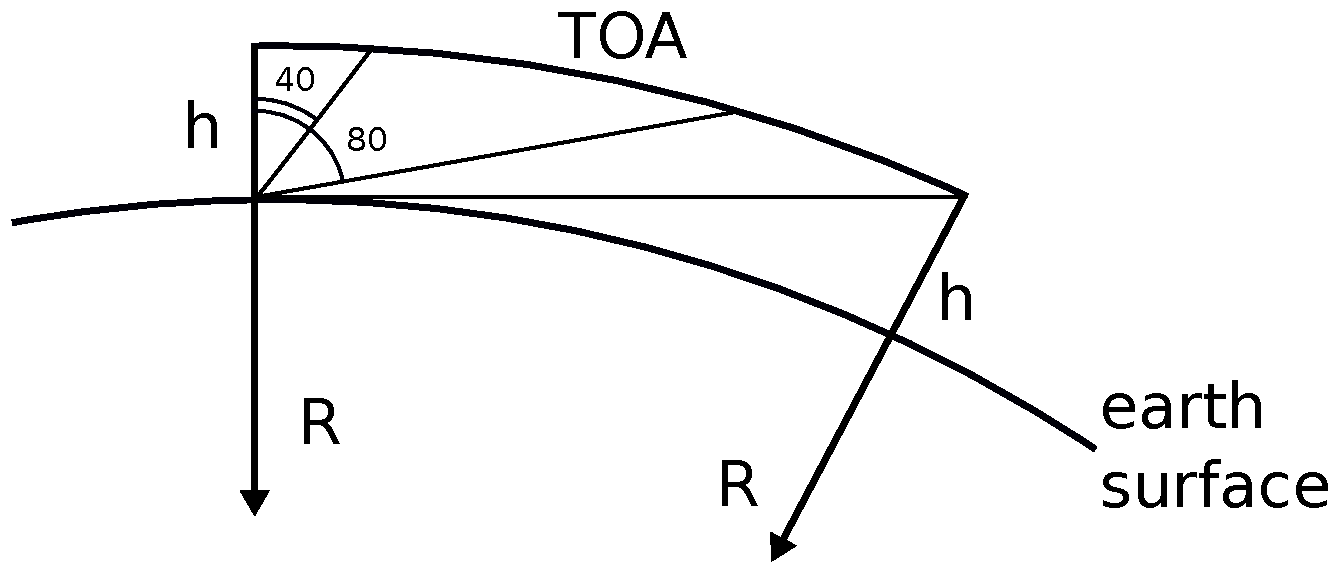
\includegraphics[width=12cm]{figures/earth_surface_toa.pdf}
	\caption{"Geometry of earth and atmosphere"}
	\label{fig:geometry}
\end{figure}

The intensity in \eqn{eqn1} is integrated along a path from the earth surface to the TOA (top of atmosphere) which is assumed to be at a heigth of $70 km$. Assuming constant $\kappa$ and $\epsilon$ in \eqn{eqn1} the solution is given by:
\begin{align}
	I(s) = I(s_0) \exp( -  \kappa (s-s_0)) + \dfrac{\epsilon}{\kappa} \left(1 - \exp( - \kappa (s-s_0))\right)
\end{align}
Because $\kappa$ and $\epsilon$ are not constant along the path from earths surface to TOA the integration is subdivided into many steps. At each step $\kappa$ and $\epsilon$ are calculated using local values of temperature and density.

In order to compute the total irradiance emanating from an area element of the surface to TOA the integration has to be done over the half sphere:
\begin{align}
	F(\theta) &= \int_0^{2 \pi} \int_0^{\pi/2} I(\theta) \sin(\theta) \cos(\theta)  d \theta d \phi \\
	  &= 2 \pi \int_0^{\theta} I(\theta) \sin(\theta) \cos(\theta) d \theta
\end{align}
The intensity $I(\theta)$ is computed at $0^o$ and two further angles (in the computations $40^o$ and $80^o$ are chosen), 
the intermediate values are interpolated by a cubic polynomial (\chap{app_a_2}).
After determining the polynomial coefficients:
\begin{align}
	a_2 &= \dfrac{(F_1 - F_0) \theta_2^3 - (F_2 - F_0) \theta_1^3}{\theta_1^2 \theta_2^3 - \theta_1^3 \theta_2^2} \\
	a_3 &= \dfrac{(F_2 - F_0) \theta_1^2 - (F_1 - F_0) \theta_2^2}{\theta_1^2 \theta_2^3 - \theta_1^3 \theta_2^2}
 \end{align}  
the integral is given by:
\begin{align}
	F(\theta) &= 2 \pi \int_0^{\theta} \left(a_0 + a_2 \theta^2 + a_3 \theta^3\right) \sin(\theta) \cos(\theta)  d \theta d \phi
\end{align}
The contributions of the different polynomial orders assuming constant $I(\theta)$ are:
\begin{align*}
	 &\int_0^{\theta} \sin(\theta) \cos(\theta) d \theta = 0.5 \\
	 &\int_0^{\theta} \theta^2 \sin(\theta) \cos(\theta) d \theta = 0.37  \\
	 &\int_0^{\theta} \theta^3 \sin(\theta) \cos(\theta) d \theta = 0.38
\end{align*}

\subsection{The HITRAN Data}

The spectroscopic $CO_2$ data where taken from the HITRAN database (\cite{hitran1}). The standard HITRAN data files use a fixed size format and information that are not used in the present report. HITRAN allows to define ones own format and data output. For easier handling the entries are separated by commas. The data rows are composed of: 
\begin{enumerate}
	\item Molecule ID, for $CO_2$ this is $2$			
 	\item Isotopologue ID, for $CO_2$ $1-9$			
 	\item the transition wavenumber $\nu$	[$cm^{-1}$]		
    \item the line strength multiplied by isotopologue abundance $S$, [$cm^{-1}/(molec \;cm^{-2}$]		
 	\item Einstein coefficient of spontaneous emission $A$ [$s^{-1}$]		
 	\item pressure line broadening coefficient by collisions with air molecules $\gamma_{air}$ [$cm^{-1} atm^{-1}$]		
 	\item pressure line broadening coefficient by collisions with $CO_2$ molecules $\gamma_{self}$ [$cm^{-1} atm^{-1}$]		
	\item energy of the lower state $E"$ [$cm^{-1}$]		
	\item temperature exponent $n_{air}$ for the air broadened HWHM			
	\item pressure shift induced by air $\delta_{air}$, referred to $p = 1 atm$ [$cm^{-1} atm^{-1}$] 		
	\item upper state degeneracy $g'$			
	\item upper state degeneracy $g"$
\end{enumerate}
In the present report wavelength $\lambda$ [$m$] and energy [$J$] is used, whereas HITRAN uses wavenumber [$cm^{-1}$]. The transition from wavelenht to wavenumber has to be done carefully.  
\begin{align*}
	\lambda_{ul}     & \leftarrow \dfrac{10^{-2}}{\nu}               & [m]                   \\
	\Delta E_{ul}    & \leftarrow \dfrac{h  c}{\lambda_{ul}}         & [J]                   \\
 	E_l              & \leftarrow h  c  \dfrac{E''}{10^{-2}}         & [J]                   \\
	E_u              & \leftarrow E_l + \Delta E_ul                  & [J]                   \\
	\gamma_a         & \leftarrow \dfrac{\gamma_{air}}{10^{-2}}  10^{-5} & \left[\dfrac{1}{m \; Pa}\right] \\
	\gamma_s         & \leftarrow \dfrac{\gamma_{self}}{10^{-2}}  10^{-5} & \left[\dfrac{1}{m \; Pa}\right] \\
	\delta_a         & \leftarrow \dfrac{\delta_{air}}{10^{-2}}  10^{-5} &
\end{align*}

The HWHM Doppler line broadening is given by: 
\begin{align*}
	\alpha_D(T) = \dfrac{\nu_{ij}}{c} \sqrt{\dfrac{2 N_A k T \ln 2}{M}}
\end{align*}
The temperature and pressure dependence of pressure broadened line width and pressure shift are defined by HITRAN as follows \cite{hitran2}: 
\begin{align*}
	\gamma(p, T) &= \left(\dfrac{T_{ref}}{T}\right)^{n_{air}}  
	               \left(  \gamma_{air} (p_{ref}, T_{ref}) (p - p_{self}) +
	                       \gamma_{self}(p_{ref}, T_{ref}) p_{self}  \right) 		 \\
	\nu_{ij}^*   &= \nu_{ij} \delta(p_{ref}) p
\end{align*}

Temperature dependent partition functions can be found at \cite{hitran3}.
\section{Results}


\begin{figure}[!ht]
 	\includegraphics[width=70mm]{results/intensity_at_toa_no_eps.png}
	\caption{Intensity at the TOA without emission.}
	\label{fig:toa1}
\end{figure}

\begin{figure}[!ht]
	\includegraphics[width=70mm]{results/intensity_at_toa_with_eps.png}
	\caption{Intensity at the TOA including emission.}
	\label{fig:toa2}
\end{figure}

\begin{figure}[!ht]
	\includegraphics[width=70mm]{results/I_vs_h.png}
	\caption{Intensity vs. height.}
	\label{fig:I_vs_h}
\end{figure}

\begin{figure}[!ht]
	\includegraphics[width=70mm]{results/absorption_coefficient.png}
	\caption{Absorption coeffient}
	\label{fig:abs_coeff}
\end{figure}

\begin{figure}[!ht]
	\includegraphics[width=70mm]{results/emission_coefficient.png}
	\caption{Emission coeffient}
	\label{fig:em_coeff}
\end{figure}

\begin{figure}[!ht]
	\includegraphics[width=70mm]{results/intensity_at_toa.png}
	\caption{Intensity at TOA}
	\label{fig:int_toa1}
\end{figure}

\begin{figure}[!ht]
	\includegraphics[width=70mm]{results/intensity_at_toa_with_eps.png}
	\caption{Intensity at TOA including emission}
	\label{fig:int_toa2}
\end{figure}


$\Delta I$ $[W/m^2]$ = I(400 bpm) - I(800 bpm) at TOA

\begin{tabular}{|c |c |c |}
	\hline
	$\Delta I$ $[W/m^2]$ & emission & \# isotopes \\
	\hline
	14.8                                     & yes      &  12         \\
	15.3                                     & yes      &  1          \\
	17.4                                     & no       &  1          \\
	12.1                                     & yes      &  1       \\
	\hline   
\end{tabular}  


\newpage
\section{Bibliography}
\printbibliography[heading=none]  
%\printbibliography[title={Bibliography}]  

\newpage
\appendix

\section{Integration of the Radiation Transfer Equation}
\label{app_a_1}

The radiation transfer equation \eqn{eqn1} is of the form:
\begin{align}
	\label{eqn_a_rte}
	\dfrac{dy}{dx} = - a y + b
\end{align}
If $a$ and $b$ are contant the solution can be written as:
\begin{align}
	y(x) = c(x) \exp( - a x)
\end{align}
Inserting into \eqn{eqn_a_rte} yields:
\begin{align}
		\dfrac{d y}{d x} = \dfrac{d c(x)}{dx} \exp( - a x) - a c(x) \exp( - a x) = - a c(x) \exp( - a x) + b
\end{align}
and further:
\begin{align}
	\dfrac{d c(x)}{dx}  = b \exp(a x)
\end{align}
This can be integrated:
\begin{align}
	d c(x) = b \exp(a x) dx
\end{align}
\begin{align}
	\int_{c_0}^c d c(x)  =  b \int_0^x \exp(a x) dx
\end{align}
\begin{align}
	c - c_0  = \dfrac{b}{a} \left(\exp(a x) - 1\right)
\end{align}
And finally:
\begin{align}
	y(x) = y(0) \exp( - a x) + \dfrac{b}{a} \left(1 - \exp( - a x)\right)
\end{align}

\section{Cubic Polynomial Interpolation}
\label{app_a_2}
\begin{align}
	y(x) = a_0 + a_1 x + a_2 x^2 +  a_3 x^3
\end{align}

With $a_0 = y(0)$ and $\dfrac{d y(0)}{d x} = 0$ it follows that $a_1 = 0$.
The coefficients $a_2$ and $a_3$ are determined by the linear system: 
\begin{align}
	y(x_1) &= y(0) + a_2 x_1^2 +  a_3 x_1^3 \\
	y(x_2) &= y(0) + a_2 x_2^2 +  a_3 x_2^3
\end{align}
which can be written as matrix equation:
\begin{align}x
	\begin{pmatrix} x_1^2 & x_1^3 \\
					x_2^2 & x_2^3 
	\end{pmatrix}
	\begin{pmatrix}	a_2 \\ a_3
	\end{pmatrix}
	=
	\begin{pmatrix} y(x_1) - y(0) \\ y(x_2) - y(0)
	\end{pmatrix}
\end{align}
Using Cramer's rule the solution is given by:
\begin{align}
 a_2 &= \dfrac{(y(x_1) - y(0)) x_2^3 - (y(x_2) - y(0)) x_1^3}{x_1^2 x_2^3 - x_1^3 x_2^2} \\
 a_3 &= \dfrac{(y(x_2) - y(0)) x_1^2 - (y(x_1) - y(0)) x_2^2}{x_1^2 x_2^3 - x_1^3 x_2^2}
\end{align}

\section{Line Shapes}

\subsection{Gaussian Lineshape}

\begin{align}
	\dfrac{\Delta \lambda}{\lambda} = \dfrac{v}{c} = \dfrac{1}{c} \sqrt{\dfrac{2 k_B T}{m}}
\end{align}

\begin{align}
	\exp(-a x_h^2) &= \dfrac{1}{2} \\
	-a x_h^2 &= \ln{\dfrac{1}{2}} \\
	a &= \dfrac{\ln{2}}{x_h^2}
\end{align}

\begin{align}
	x_h = x_{hwhm} = \Delta \lambda
\end{align}

\begin{align}
	a &= \dfrac{\ln{2}}{\Delta \lambda^2}
\end{align}

\begin{align}
	\int \exp\left(- \dfrac{\ln{2}}{\Delta \lambda^2} x^2\right) dx = \sqrt{\dfrac{\pi}{a}}
\end{align}

\begin{align}
	\sqrt{\dfrac{a}{\pi}} \int \exp\left(- \dfrac{\ln{2}}{\Delta \lambda^2} x^2\right) dx = 1
\end{align}

\begin{align}
	\sqrt{\dfrac{\dfrac{\ln{2}}{\Delta \lambda^2}}{\pi}} \int \exp\left(- \dfrac{\ln{2}}{\Delta \lambda^2} x^2\right) dx = 1
\end{align}

\begin{align}
	&\Delta \lambda = \dfrac{1}{c} \sqrt{\dfrac{2 k_B T}{m}} \lambda \\
	&\sqrt{\dfrac{\ln{2}}{\pi \Delta \lambda^2}} \int \exp\left(- \dfrac{\ln{2}}{\Delta \lambda^2} (\lambda - \lambda_0)^2\right) dx = 1
\end{align}

\subsection{Lorentz Lineshape}

\begin{align}
	L(\nu) = \dfrac{a^2}{ (\nu - \nu_0)^2 + a^2}
\end{align}

\begin{align}
	L(\nu_0) = 1
\end{align}

\begin{align}
	L(\nu_h) = 1/2  = \dfrac{a^2}{ (\nu_h - \nu_0)^2 + a^2}
\end{align}

\begin{align}
	 (\nu_h - \nu_0)^2 + a^2 = 2 a^2
\end{align}

\begin{align}
	(\nu_h - \nu_0) = \Delta \nu = a
\end{align}

\begin{align}
	L(\nu) = \dfrac{\Delta \nu^2}{ (\nu - \nu_0)^2 + \Delta \nu^2}
\end{align}

\begin{align}
	L(\lambda) = \dfrac{b^2}{ c^2(1/\lambda - 1/\lambda_0)^2 + b^2}
\end{align}

\begin{align}
	L(\lambda) = \dfrac{b^2}{ c^2 \left(\dfrac{\lambda - \lambda_0}{\lambda  \lambda_0}\right)^2 + b^2}
\end{align}

\begin{align}
	L(\lambda) = \dfrac{b^2 \lambda^2 \lambda_0^2}{c^2}
				\dfrac{1}{\left(\lambda - \lambda_0\right)^2 + \lambda^2 \lambda_0^2 b^2/c^2}
\end{align}

\begin{align}
	L(\lambda_0) = 1
\end{align}

\begin{align}
	L(\lambda_h) = \dfrac{1}{2} = \dfrac{b^2 \lambda_h^2 \lambda_0^2}{c^2}
\dfrac{1}{\left(\lambda_h - \lambda_0\right)^2 + \lambda_h^2 \lambda_0^2 b^2/c^2}
\end{align}

\begin{align}
	 2 \dfrac{b^2 \lambda_h^2 \lambda_0^2}{c^2}
				= \left(\lambda_h - \lambda_0\right)^2 + \lambda_h^2 \lambda_0^2 b^2/c^2
\end{align}

\begin{align}
	\dfrac{b^2 \lambda_h^2 \lambda_0^2}{c^2}
		= \left(\lambda_h - \lambda_0\right)^2
\end{align}

\begin{align}
	\dfrac{b^2}{c^2} = \left(\lambda_h - \lambda_0\right)^2 \dfrac{1}{\lambda_h^2 \lambda_0^2}
\end{align}

\begin{align}
	L = \left(\lambda_h - \lambda_0\right)^2 \dfrac{1}{\left(\lambda - \lambda_0\right)^2 + \left(\lambda_h - \lambda_0\right)^2}
\end{align}

\begin{align}
	\Delta \lambda_{hwhm} = \lambda - \lambda_0
\end{align}

\begin{align}
	L =   \dfrac{ \Delta \lambda^2}{\left(\lambda - \lambda_0\right)^2 + \Delta \lambda^2}
\end{align}

\begin{align}
   \int_{-\infty}^{-\infty} \dfrac{1}{1 + x^2} dx = \arctan(\infty) - \arctan(-\infty) = \pi
\end{align}


\begin{align}
	x &= \dfrac{\left(\lambda - \lambda_0\right)}{ \Delta \lambda} \\
	dx &= \dfrac{1}{\Delta \lambda} d\lambda
\end{align}

\begin{align}
	L =   \dfrac{\dfrac{1}{\pi} \Delta \lambda}{\left(\lambda - \lambda_0\right)^2 + \Delta \lambda^2}
\end{align}

\begin{align}
	L =  \dfrac{1}{\pi} \dfrac{\Delta \lambda}{\left(\lambda - \lambda_0\right)^2 + \Delta \lambda^2}
\end{align}

\begin{align}
	\int \dfrac{1}{\pi} \dfrac{\Delta \lambda}{\left(\lambda - \lambda_0\right)^2 + \Delta \lambda^2} d\lambda = 1
\end{align}

\begin{align}
	\int \dfrac{1}{\pi} \dfrac{\Delta \lambda}{\left(\lambda - \lambda_0\right)^2 + \Delta \lambda^2} d\lambda = 1
\end{align}




\newpage
%\section{Line Strength}

\begin{align}
	\left(S/d\right)_n  = \dfrac{1}{\Delta \nu} \sum_j S_j(T_n)
\end{align}

\begin{align}
	S_j(T_n)  = \dfrac{Q_r(T_s) Q_v(T_s)}{Q_r(T_n) Q_v(T_n)} \dfrac{1 - \exp(-h \nu_j / k_B/T_s)}{1 - \exp(-h \nu_j / k_B/T_n)}
		\exp\left(\dfrac{E_j T_n T_s}{k_B T_0 T_s}\right) S_j(T_s)
\end{align}

\begin{align}
	\gamma(T,p) = \gamma(T_0,p_0) \dfrac{p}{p_0} \left(\dfrac{T_0}{T}\right)^{x_m}
\end{align}
\begin{align}
	T_0 &= 273.15 K \\
	p_0 &= 1013.25 mbar \\
	x_m &= 3/4
\end{align}



\subsection{Radiation Transfer Equation in Frequency Space}

\begin{align}
&\dfrac{d I_{\nu}}{ds} = - \kappa_{\nu} I_{\nu} + \epsilon_{\nu} \\
&I_{\nu}        : \left[\dfrac{W}{m^2 \; sr \; Hz}\right] \\
&\epsilon_{\nu} : \left[\dfrac{W}{m^3 \; sr \; Hz}\right] \\
&\kappa_{\nu}   : \left[\dfrac{1}{m}\right]
\end{align}

\begin{align}
\epsilon_{\nu} = \dfrac{1}{4 \pi} h \nu N_u A_{ul} f(\nu) \;\;\; , \;\;\; \left[\dfrac{W}{m^3 sr Hz}\right]
\end{align}

\begin{align}
\int f(\nu) d\nu = 1
\end{align}

\subsubsection{Equilibrium}
\begin{align}
\dfrac{d I_{\nu}}{ds} = - \kappa_{\nu} I_{\nu} + \epsilon_{\nu} = 0
\end{align}

\subsubsection{Planck}
\begin{align}
&u_{\nu} = \dfrac{4 \pi \;\; 2 h \nu^3}{c^3}  \dfrac{1}{\exp\left(\dfrac{h \nu}{k_B T}\right) - 1} \;\;\; , \;\;\; \left[\dfrac{J}{m^3 Hz}\right]
\end{align}
with:
\begin{align}
I_{\nu} = \dfrac{u_{\nu}}{4 \pi} c
\end{align}
\begin{align}
I_{\nu} = \dfrac{2 h \nu^3}{c^2}  \dfrac{1}{\exp\left(\dfrac{h\nu}{k_B T}\right) - 1} \;\;\; , \;\;\; \left[\dfrac{W}{m^2 sr Hz}\right]
\end{align}

\begin{align}
\kappa_{\nu} = \dfrac{1}{4 \pi} h \nu N_u A_{ul} f(\nu) \;\; \left(\exp\left(\dfrac{h \nu}{k_B T}\right) - 1\right) \dfrac{c^2}{2 h \nu^3}   \;\;\; , \;\;\; \left[\dfrac{1}{m}\right]
\end{align}

\begin{align}
\kappa_{\nu} = \dfrac{1}{8 \pi} \dfrac{c^2}{\nu^2} N_u A_{ul} \left(\exp\left(\dfrac{h \nu}{k_B T}\right) - 1\right) f(\nu)  \;\;\; , \;\;\; \left[\dfrac{1}{m}\right]
\end{align}


\begin{align}
\kappa_\nu = \dfrac{h \nu}{c} \left(N_l B_{lu} - N_u B_{ul}\right) f(\nu)
\end{align}

\begin{align} 
\kappa_\nu = \dfrac{h \nu}{c} N \left(g_l \exp\left(-\dfrac{E_l}{k_B T}\right) B_{lu} - g_u\exp\left(-\dfrac{E_u}{k_B T}\right) B_{ul}\right) f(\nu)
\end{align}

\begin{align}
\kappa_\nu = \dfrac{h \nu}{c} N \exp\left(-\dfrac{E_u}{k_B T}\right) \left(\exp\left(-\dfrac{(E_u-E_l)}{k_B T}\right) 
g_l B_{lu} - g_u B_{ul}\right) f(\nu)
\end{align}

\begin{align}
g_l B_{lu} = g_u B_{ul}
\end{align}

\begin{align}
\kappa_\nu = \dfrac{h \nu}{c} N g_u B_{ul} \exp\left(-\dfrac{E_u}{k_B T}\right) 
\left(\exp\left(-\dfrac{h \nu}{k_B T}\right) - 1\right) f(\nu)
\end{align}

\begin{align}
\kappa_\nu = \dfrac{h \nu}{c} B_{ul} N_u \left(\exp\left(-\dfrac{h \nu}{k_B T}\right) - 1\right) f(\nu) \;\;\; , \;\;\; \left[\dfrac{1}{m}\right]
\end{align}

\begin{align}
\dfrac{h \nu}{c} B_{ul} N_u = \dfrac{1}{8 \pi} \dfrac{c^2}{\nu^2} N_u A_{ul}
\end{align}

\begin{align}
B_{ul} = \dfrac{1}{8 \pi} \dfrac{c^3}{h \nu^3} A_{ul} \;\;\; , \;\;\; \left[\dfrac{m^3}{J s^2}\right]
\end{align}


\subsection{Radiation Transfer Equation in Wavelength Space}

\begin{align}
I_\lambda = \dfrac{2 \pi h c^2}{\lambda^5} \dfrac{1}{\exp\left(\dfrac{h c}{\lambda k_B T}\right) - 1}
\end{align}

\begin{align}
I = \int I_{\lambda} d\lambda
\end{align}

\begin{align}
I_{\nu} d\nu = I_{\lambda} d\lambda
\end{align}
\begin{align}
&\nu = \dfrac{c}{\lambda} \\
&d\nu = -\dfrac{c}{\lambda^2} d\lambda \\
&I_{\nu} \dfrac{c}{\lambda^2} d\lambda = I_{\lambda} d\lambda \\
&I_{\nu} \dfrac{c}{\lambda^2} = I_{\lambda} \\
&I_{\nu} = I_{\lambda} \dfrac{\lambda^2}{c}
\end{align}


\begin{align}
\dfrac{d I_{\lambda}}{ds} = - \kappa_\lambda I_{\lambda} + 	\epsilon_\lambda
\end{align}

\begin{align}
\kappa_\lambda = \dfrac{h}{\lambda_0} \left(N_l B_{lu} - N_u B_{ul}\right) f(\lambda) \dfrac{\lambda^2}{c}
\end{align}

\begin{align}
\kappa_\lambda = \dfrac{h \lambda}{c} \left(N_l B_{lu} - N_u B_{ul}\right) f(\lambda) 
\;\;\; , \;\;\; \left[\dfrac{1}{m}\right]
\end{align}

\begin{align}
\epsilon_\nu f(\nu) d \nu &= 	\epsilon_\lambda f(\lambda)  d\lambda \\
f(\nu) d \nu &= 	f(\lambda)  d\lambda \\
\epsilon_\nu &= \epsilon_\lambda \\
\epsilon_\lambda &= \dfrac{1}{4 \pi} \dfrac{h c}{\lambda} N_u A_{ul} f(\lambda) 
\;\;\; , \;\;\; \left[\dfrac{W}{m^3 sr \;m}\right]
\end{align}

\begin{align}
\int f_{\lambda} d\lambda = 1
\end{align}

\begin{align}
B_{ul} = A_{ul} \dfrac{\lambda^3}{8 \pi h} \;\;\; , \;\;\; \left[\dfrac{m^3}{J s^2}\right]
\end{align}

\begin{align}
B_{lu} = \dfrac{g_u}{g_l} B_{ul}
\end{align}

\begin{align}
<\epsilon> = \int \epsilon_{\lambda}(\lambda) d\lambda
\end{align}

\begin{align}
<\kappa> = \dfrac{\int \kappa_{\lambda}(\lambda) I_{\lambda}(\lambda) d\lambda}{\int I_{\lambda}(\lambda) d\lambda}
\end{align}

In thermal equilibrium the intensity is constant:
\begin{align}
&\dfrac{d I_{\lambda}}{ds} = - \kappa_\lambda I_{\lambda} + 	\epsilon_\lambda = 0 \\
&\kappa_\lambda = \dfrac{\epsilon_\lambda}{I_{\lambda}}
\end{align}

and the intensity is given by Planck's formula:
\begin{align}
I_\lambda = \dfrac{2 h c^2}{\lambda^5} \dfrac{1}{\exp\left(\dfrac{h c}{\lambda k_B T}\right) - 1}
\end{align}

With this the net absorption coefficient $\kappa_\lambda$ is:
\begin{align}
\kappa_\lambda = \dfrac{\dfrac{1}{4 \pi} \dfrac{h c}{\lambda} N_u A_{ul} f(\lambda) }{\dfrac{2 h c^2}{\lambda^5} \dfrac{1}{\exp\left(\dfrac{h c}{\lambda k_B T}\right) - 1}} =
\dfrac{\lambda^4 }{8 \pi c} A_{ul} N_u  \left(\exp\left(\dfrac{h c}{\lambda k_B T}\right) - 1\right) f(\lambda)
\end{align}
The densities of upper and lower state are given by:
\begin{align}
N_u &= N \dfrac{g_u}{Q(T)} \exp\left(- \dfrac{E_u}{k_B T} \right) \\
N_l &= N \dfrac{g_l}{Q(T)} \exp\left(- \dfrac{E_l}{k_B T} \right)
\end{align}
which yields:
\begin{align}
\kappa_\lambda  =
\dfrac{\lambda^4 }{8 \pi c} A_{ul} N \dfrac{g_u}{Q(T)}
\left( \exp\left(-\dfrac{E_l}{\lambda k_B T}\right) - \exp\left(-\dfrac{E_u}{\lambda k_B T}\right) \right) f(\lambda)
\end{align}
With:
\begin{align}
B_{ul} &= \dfrac{1}{8 \pi} \dfrac{\lambda^3}{h} A_{ul} \;\;\; , \;\;\; \left[\dfrac{m^3}{J s^2}\right] \\
B_{lu} &= \dfrac{g_u}{g_l} B_{ul}
\end{align}
this becomes
\begin{align}
\kappa_\lambda  =
\dfrac{h \lambda }{c}  
\left(  B_{ul} N \dfrac{g_u}{Q(T)} \exp\left(-\dfrac{E_l}{\lambda k_B T}\right) - 
B_{lu} N \dfrac{g_l}{Q(T)} \exp\left(-\dfrac{E_u}{\lambda k_B T}\right) \right) f(\lambda)
\end{align}
and:

\begin{align}
\kappa_\lambda  = \dfrac{h \lambda }{c}  
\left(  B_{lu} N_l -  B_{ul} N_u \right) f(\lambda)
\end{align}


\section{Random}

\begin{align}
	g_1 B_{12} = g_2 B_{21}
\end{align}

\begin{align}
	A_{21} = 8 \pi h \nu^3 B_{21}
\end{align}

\begin{align}
	\kappa(\nu - \nu_0)	= (N_1 B_{12} - N_2 B_{21}) \dfrac{h \nu_0}{c} f(\nu - \nu_0)
\end{align}

\begin{align}
	S = \dfrac{1}{N} (N_1 B_{12} - N_2 B_{21}) \dfrac{h \nu_0}{c}
\end{align}

\begin{align}
	S = \dfrac{g_2}{Q_{tot}(T)} \dfrac{A_{21}}{8  \pi c \nu_0^2} \exp(- E_1 / k_BT)
		(1 - \exp(- h \nu_0 / k_BT))
\end{align}

Power per unit area

\begin{align}
	B(\nu, T) = \dfrac{2 \pi h \nu^3}{c^2} \dfrac{1}{ \exp(h \nu /  k_B T) - 1}
\end{align}


\begin{align}
	\dfrac{d I_{\nu}}{dz} = -\alpha_{\nu}	 (I_{\nu} - B(\nu, T))
\end{align}

\begin{align}
	\alpha_{\nu} = N \sigma_{\nu}
\end{align}

\begin{align}
	\sigma_{\nu} = \sum_i \dfrac{S_i}{\pi} \dfrac{\gamma_i}{\gamma_i^2 + (\nu - \nu_i)^2}
\end{align}


\begin{align}
	B_{ul} = A_{ul} \dfrac{8 \pi h \nu_0^3}{c^3	}
\end{align}

\begin{align}
	\epsilon_{\nu} = \dfrac{h \nu}{4 \pi} N_u A_{ul} f(\nu)
\end{align}
\begin{align}
	\kappa_{\nu} = \dfrac{h \nu_0}{c} (N_l B_{lu} - N_u B_{ul}) f(\nu)
\end{align}
\begin{align}
	\dfrac{d I_{\nu}}{ds} = - \kappa_{\nu} I_{\nu} + \epsilon_{\nu}
\end{align}

Equlibrium
\begin{align}
	\dfrac{d I_{\nu}}{ds} = - \kappa_{\nu} I_{\nu} + \epsilon_{\nu} = 0
\end{align}

\begin{align}
	I_{\nu} = \dfrac{2 h \nu^3}{c^2}  \dfrac{1}{\exp(h \nu /  k_B T) - 1}
\end{align}

\begin{align}
	u_{\nu} = \dfrac{4 \pi 2 h \nu^3}{c^3}  \dfrac{1}{\exp(h \nu /  k_B T) - 1}
\end{align}

\begin{align}
	I_{\nu} = \dfrac{u_{\nu}}{4 \pi} c
\end{align}

\begin{align}
	\kappa_{\nu} I_{\nu} = \epsilon_{\nu} = \dfrac{h \nu}{4 \pi} N_u A_{ul}
\end{align}

\begin{align}
	\kappa_{\nu} = \dfrac{h \nu}{4 \pi} N_u A_{ul} (\exp(h \nu /  k_B T) - 1) \dfrac{c^2}{2 h \nu^3}
\end{align}


\begin{align}
	I_\nu = \dfrac{2 \pi h \nu^3}{c^2} \dfrac{1}{\exp\left(\dfrac{h \nu}{k_B T}\right) - 1}
\end{align}

\begin{align}
	I = \int I_{\nu} d\nu
\end{align}

\begin{align}
	\dfrac{d I_{\nu}}{ds} = - \kappa_\nu I_{\nu} + 	\epsilon_\nu
\end{align}

\begin{align}
	\kappa_\nu = \dfrac{h \nu_0}{c} \left(N_l B_{lu} - N_u B_{ul}\right) f(\nu)
\end{align}

\begin{align}
	\epsilon_\nu = \dfrac{1}{4 \pi} h \nu_0 N_u A_{ul}  f(\nu)
\end{align}

\begin{align}
	\int f_{\nu} d\nu = 1
\end{align}

\begin{align}
	B_{ul} = A_{ul} \dfrac{c^3}{8 \pi h \nu^3}
\end{align}

\begin{align}
	B_{lu} = \dfrac{g_u}{g_l} B_{ul}
\end{align}


\section{Coments on the Article Reinhart}
\subsection{Difference between the Radiation Transfer Equation and Reinhart Equation 9}

\subsubsection{Radiation Transfer Equation}

\begin{align}
	\dfrac{d I(\lambda)}{ds} = - I(\lambda) \kappa(\lambda)
\end{align}
\begin{align}
	\dfrac{I_{abs}}{I_0} = \int_{\lambda_1}^{\lambda_2} \left(1 - exp(-\kappa(\lambda) z)\right) d \lambda
\end{align}

\subsubsection{Reinhart Equationn 9}

\begin{align}
	\dfrac{I_{abs}}{I_0} = \sum_i (1 - \exp(-\kappa_i z)) \Delta \lambda_i
\end{align}

\subsubsection{Simple Model}

Two partially overlapping lines with rectangle shaped line shapes:
\begin{figure}[ht]
	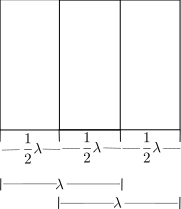
\includegraphics[width=6cm]{figures/overlappinglines2.png}
	\caption{Two overlapping lines with rectangle line shape functions}
	\label{fig:overlappinglines}
\end{figure}

Reinhart:
\begin{align}
	\Delta J_1 &= \left(1 - \exp( - \kappa_1 z)\right) \Delta \lambda \\
	\Delta J_2 &= \left(1 - \exp( - \kappa_2 z)\right) \Delta \lambda 
\end{align}
\begin{align}
	A = \dfrac{\Delta J_1 + \Delta J_2}{\Delta \lambda} = \left(1 - \exp( - \kappa_1 z)\right) + \left(1 - \exp( - \kappa_2 z)\right)
\end{align}
Radiation transfer solution :
\begin{align}
	\Delta I_1 &= \left(1 - \exp( - \kappa_1 z)\right) \dfrac{\Delta \lambda}{2} \\
	\Delta I_2 &=  \left(1 - \exp( - \kappa_2 z)\right) \dfrac{\Delta \lambda}{2} \\
	\Delta I_{12} &= \left(1 - \exp( - \kappa_1 z - \kappa_2 z)\right) \dfrac{\Delta \lambda}{2}
\end{align}
\begin{align}
	B = \dfrac{\Delta I_1 + \Delta I_2 + \Delta I_{12}}{I_0 \Delta \lambda} =
			& \dfrac{1}{2} \left(1 - \exp( - \kappa_1 z)\right) +  \\
			& \dfrac{1}{2} \left(1 - \exp( - \kappa_2 z)\right) + \\ 
			& \dfrac{1}{2} \left(1 - \exp( - \kappa_1 z - \kappa_2 z)\right) 
\end{align}
The difference is:
\begin{align}
	2(A - B) &= \left(1 - \exp( - \kappa_1 z)\right) + \left(1 - \exp( - \kappa_2 z)\right) -
	\left(1 - \exp( - \kappa_1 z - \kappa_2 z\right) \\
	         &= 1  + \exp(- \kappa_1 z - \kappa_2 z) - \exp( - \kappa_1 z) - \exp( - \kappa_2 z)
\end{align}
In case of $\kappa_1 \gg 1$ and $\kappa_2 \gg 1$ this yields: 
\begin{align}
	(\Delta J_1 + \Delta J_2) - (\Delta I_1 + \Delta I_2 + \Delta I_{12})=
	I_0 \dfrac{\Delta \lambda}{2}
\end{align}
That means the absorption of the overlapping region is counted twice.
%\subsection{Difference between the Radiation Transfer Equation and Reinhart Equation 9}

\subsubsection{Radiation Transfer Equation}

\begin{align}
	\dfrac{d I(\lambda)}{ds} = - I(\lambda) \kappa(\lambda)
\end{align}
\begin{align}
	\dfrac{I_{abs}}{I_0} = \int_{\lambda_1}^{\lambda_2} \left(1 - exp(-\kappa(\lambda) z)\right) d \lambda
\end{align}

\subsubsection{Reinhart Equationn 9}

\begin{align}
	\dfrac{I_{abs}}{I_0} = \sum_i (1 - \exp(-\kappa_i z)) \Delta \lambda_i
\end{align}

\subsubsection{Simple Model}

Two partially overlapping lines with rectangle shaped line shapes:
\begin{figure}[ht]
	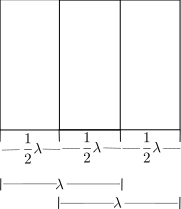
\includegraphics[width=6cm]{figures/overlappinglines2.png}
	\caption{Two overlapping lines with rectangle line shape functions}
	\label{fig:overlappinglines}
\end{figure}

Reinhart:
\begin{align}
	\Delta J_1 &= \left(1 - \exp( - \kappa_1 z)\right) \Delta \lambda \\
	\Delta J_2 &= \left(1 - \exp( - \kappa_2 z)\right) \Delta \lambda 
\end{align}
\begin{align}
	A = \dfrac{\Delta J_1 + \Delta J_2}{\Delta \lambda} = \left(1 - \exp( - \kappa_1 z)\right) + \left(1 - \exp( - \kappa_2 z)\right)
\end{align}
Radiation transfer solution :
\begin{align}
	\Delta I_1 &= \left(1 - \exp( - \kappa_1 z)\right) \dfrac{\Delta \lambda}{2} \\
	\Delta I_2 &=  \left(1 - \exp( - \kappa_2 z)\right) \dfrac{\Delta \lambda}{2} \\
	\Delta I_{12} &= \left(1 - \exp( - \kappa_1 z - \kappa_2 z)\right) \dfrac{\Delta \lambda}{2}
\end{align}
\begin{align}
	B = \dfrac{\Delta I_1 + \Delta I_2 + \Delta I_{12}}{I_0 \Delta \lambda} =
			& \dfrac{1}{2} \left(1 - \exp( - \kappa_1 z)\right) +  \\
			& \dfrac{1}{2} \left(1 - \exp( - \kappa_2 z)\right) + \\ 
			& \dfrac{1}{2} \left(1 - \exp( - \kappa_1 z - \kappa_2 z)\right) 
\end{align}
The difference is:
\begin{align}
	2(A - B) &= \left(1 - \exp( - \kappa_1 z)\right) + \left(1 - \exp( - \kappa_2 z)\right) -
	\left(1 - \exp( - \kappa_1 z - \kappa_2 z\right) \\
	         &= 1  + \exp(- \kappa_1 z - \kappa_2 z) - \exp( - \kappa_1 z) - \exp( - \kappa_2 z)
\end{align}
In case of $\kappa_1 \gg 1$ and $\kappa_2 \gg 1$ this yields: 
\begin{align}
	(\Delta J_1 + \Delta J_2) - (\Delta I_1 + \Delta I_2 + \Delta I_{12})=
	I_0 \dfrac{\Delta \lambda}{2}
\end{align}
That means the absorption of the overlapping region is counted twice.


\end{document}
